% !TeX spellcheck = de
\documentclass[10pt,a4paper]{beamer}

\usepackage[german]{babel} % deutsch und deutsche Rechtschreibung
\usepackage[utf8]{inputenc}
\usepackage[T1]{fontenc} % Umlaute und deutsches Trennen
\usepackage{amsmath}
\usepackage{amsfonts}
\usepackage{amssymb}
\usepackage{graphicx}
\usepackage{url}
\usepackage{color}
\usepackage{listings}

\DeclareGraphicsExtensions{.pdf,.jpeg,.png}
\graphicspath{{img/}}

\newcommand{\ent}{\mathrel{\widehat{=}}}
\newcommand{\hr}{\noindent\makebox[\linewidth]{\rule{\paperwidth}{0.4pt}}\vspace{0.8em}\\}

\newenvironment{card}[1]
  {\begin{frame}[fragile,environment=card]#1}
  {\end{frame}}
  
\lstset{
	keepspaces=true,
	%columns=flexible,
	keywordstyle=\color{blue},
	stringstyle=\color{red!40!black},
	commentstyle=\color{green!40!black},
	identifierstyle=\color{blue!40!black}
}

\begin{document}
\begin{card}
	\frametitle{Übung 2: Konzepte Abstraktion}
	\url{http://people.f4.htw-berlin.de/~hebold/htw/pka/exercises/konzepte-Abstraktion.pdf}
\end{card}

\begin{card}
	Nennen Sie mindestens 3 Gründe für Abstraktion.
	\hr
	\begin{enumerate}
	\item Wiederverwendbarkeit von allgemeinen Problemlösungen
	\item Klassifizieren von Problemen, erkennen der Struktur
	\item Allgemeine Lösung zu detaillierten Problemen (Kompression)
	\item Vereinfachung
	\end{enumerate}
\end{card}

\begin{card}
	Inwiefern wird beim Programmieren ganz generell abstrahiert?
	\hr
	\begin{enumerate}
	\item OOP $\Leftrightarrow$ reelle Welt, internes Modell als Abstraktion
	\item Abstraktion von Problembeispielen auf Programmcode
	\item Programme $\Leftrightarrow$ Prozessen, insbesondere beim Debuggen ständiger Kontextwechsel
	\end{enumerate}
\end{card}

\begin{card}
	Inwiefern wird bei der \textbf{strukturierten} Programmierung abstrahiert?
	\hr
	\begin{enumerate}
	\item if, for, while-Konstrukte ersetzen Sprungbefehle\\
		Beispiel: labels mit goto (?)
	\end{enumerate}
\end{card}

\begin{card}
	Inwiefern wird bei der \textbf{prozeduralen} Programmierung abstrahiert?
	\hr
	\begin{enumerate}
	\item parametrisierte Prozeduren ersetzen alle Werte-Kombinationen beim Aufruf
	\end{enumerate}
	Beispiel:
\end{card}

\begin{card}
	Inwiefern wird bei der \textbf{modularen} Programmierung abstrahiert?
	\hr
	\begin{enumerate}
	\item statische Werte, d.h. kein Zustand
	\item Blackbox, Implementierung unbekannt\\
		Beispiel: sort(array[] field)
	\end{enumerate}

\end{card}

\begin{card}
	Inwiefern wird bei der \textbf{objekt-orientierten} Programmierung abstrahiert?
	\hr
	\begin{enumerate}
	\item Vererbung von generischen Datentypen
	\item Polymorphismus, dynamisches Binden
	\end{enumerate}
	Beispiel:
\end{card}

\begin{card}
	Inwiefern wird bei der \textbf{funktionalen} Programmierung abstrahiert?
	\hr
	\begin{enumerate}
	\item Nur Funktionen und Rückgabewerte, keine Datentypen, bzw. Objekte
	\item Überladen von Funktionen
	\end{enumerate}
	Beispiel:
\end{card}

\begin{card}
	Inwiefern wird bei der Programmierung abstrakter Datentypen abstrahiert?
	\hr
	\begin{enumerate}
	\item Lists, Arrays als Abstraktion, vgl. Gruppe (Math.)\\
		Beispiel: new ArrayList<Integer>().get(0)
	\end{enumerate}
\end{card}

\begin{card}
	Beim Abstraktionskonzept wird auf verschiedenen konkreten Objekten mit einem Namen referiert, wobei die Besonderheiten unberücksichtigt bleiben - von diesen wird abstrahiert.\\
	Bei der Konkretisierung wird umgekehrt einem Namen ein bestimmtes konkretes Objekt zugeordnet - der Name wird gebunden.\\
	Wann erfolgt im Rahmen der Programmierung die Konkretisierung, d.h. die Bindung	eines Namens?
	\hr
	Bei der Zuweisung, zur Laufzeit: Namen = Konstant\\
	Beispiel:
	\begin{lstlisting}[language=Java]
	// Abstraktion:
	List x = new ArrayList();
	// Konkretisierung:
	void doSth(List x) {ArrayList y=(ArrayList)x;}
	\end{lstlisting}
\end{card}

\begin{card}
	Imperative Programmierung:\\
	Von was wird durch einen Variablennamen abstrahiert?
	\hr
	Vom Wert, da nur die Referenz auf den Wert benutzt wird\\
	Beispiel
\end{card}

\begin{card}
	Imperative Programmierung:\\
	Von was wird durch Pointer abstrahiert?
	\hr
	Von der Speicheradresse\\
	Beispiel
\end{card}

\begin{card}
	Imperative Programmierung:\\
	Von was wird durch eine Initialisierung \texttt{int i=42} abstrahiert?
	\hr
	Von der Speicherdarstellung	\\
	Beispiel: Big Indian/ Little Indian(?)
\end{card}

\begin{card}
	Imperative Programmierung:\\
	Von was wird durch eine Zuweisung abstrahiert?
	\hr
	Von allen verschiedenen Zuweisungsoperatoren\\
	Beispiel
\end{card}

\begin{card}
	Imperative Programmierung:\\
	Von was wird durch 
	\begin{enumerate}
	\item if-Abfrage
	\item for-Schleife \texttt{for(int i=0;i<a;i++) block} 
	\item while-Schleife
	\end{enumerate}
	abstrahiert?
	\hr
	goto + label\\
	Beispiel
\end{card}

\begin{card}
	Imperative Programmierung:\\
	Von was wird durch eine Prozedur (void) abstrahiert?
	\hr
	Von der Implementierung\\
	Beispiel
\end{card}

\begin{card}
	Imperative Programmierung:\\
	Von was wird durch eine Funktion (non-void) abstrahiert?
	\hr
	Von der Implementierung\\
	der Rückgabewert abstrahiert von der Funktion\\
	Beispiel
\end{card}

\begin{card}
	Imperative Programmierung:\\
	Von was wird in C und C++ und Java durch den abstrakten Datentyp Array abstrahiert?
	\hr
	C und C++: Von Pointern, Beispiel: \begin{lstlisting}
		
		\end{lstlisting}
	
	Java: Von Referenzen, Beispiel: \begin{lstlisting}
	{"a", "b", "c"}.get(0)
	\end{lstlisting}
	
\end{card}

\begin{card}
	Imperative Programmierung:\\
	Funktionen werden in C, C++ und Java durch Aufrufe zur Laufzeit konkretisiert. Signatur und Methode sind die Abstraktionen. Zusätzlich bietet C++ Funktionen mit default Parametern. Was bedeuten diese für Abstraktion und Konkretisierung?
	\hr
	???
\end{card}

\begin{card}
	Imperative Programmierung:\\
	Von was wird in C++ durch eine inline-Funktion abstrahiert?
	\hr
	Wie Makros als Textersetzung ohne Stack, jedoch wie Funktion mit Auswertung
\end{card}

\begin{card}
	Objektorientierte Programmierung:\\
	Von was wird in Java durch eine Referenz \texttt{Type ref} abstrahiert?
	\hr
	\texttt{Type}: Für alle Objekt-Typen und deren Ableitung von Type\\
	\texttt{ref}: Abstraktion der Objekte, aber nicht vom Objekt selbst
\end{card}

\begin{card}
	Objektorientierte Programmierung:\\
	Die meisten objektorientierter Sprachen verfügen über primitive Datentypen wie z.B. int. Warum haben diese primitiven Datentypen aus der Warte des Abstraktionskonzepts einen Sonderstatus?
	\hr
	Call-by-Value: Passen direkt in Referenzspeicherbereich, keine Kapselung notwendig
\end{card}

\begin{card}
	Objektorientierte Programmierung:\\
	Was wird durch die ausschließliche Verwendung von Klassen, Objekten und Referenzen, d.h. durch die Streichung der primitiven Datentypen, im Sinne des Abstraktionskonzepts erreicht?
	\hr
	Kontinuität
\end{card}

\begin{card}
	Objektorientierte Programmierung:\\
	C++ und Java kennen die Möglichkeit des \textbf{overriding}. Inwiefern handelt es sich um eine Abstraktion? D.h. von welchen konkrete Elementen wird abstrahiert? 
	\hr
	Von der Implementierung der Objekt-Methode
\end{card}

\begin{card}
	Objektorientierte Programmierung:\\
	Mehrfachvererbung ist in Java bei Klassen nicht zugelassen. 
	\begin{enumerate}
	\item Nennen Sie eine Begründung im Rahmen des Abstraktionsprinzips.
	\item Wieso ist Mehrfachvererbung bei Interfaces zugelassen?
	\item Wie löst C++ die genannten Probleme?
	\end{enumerate}
	\hr
	\begin{enumerate}
	\item Overriding von Methoden ist somit eindeutig
	\item Es steckt keine konkrete Implementierung dahinter
	\item Durch die Reihenfolge der Vererbung
	\end{enumerate}
\end{card}

\begin{card}
	Objektorientierte Programmierung:\\
	Inwiefern handelt es sich bei der Definition von superclasses um eine Abstraktion?
	\hr
	\begin{enumerate}
	\item Verallgemeinerung mit weniger Eigenschaften
	\item Allgemeingültige Klasse für alle Unterklassen
	\item Generalisierung Richtung Oberklasse
	\end{enumerate}
\end{card}

\begin{card}
	Funktionale Programmierung:\\
	Inline-Funktionen sind Teil der meisten funktionalen Sprachen. Beschreiben Sie im Rahmen des Abstraktionskonzepts das Problem mit rekursiv definierten (inline-) Funktionen.
	\hr
	Nur 1 Rückgabewert\\
	Beispiel:
\end{card}

\begin{card}
	Funktionale Programmierung:\\
	Inwiefern kann man sagen, dass in rein funktionalen Sprachen auf einer höheren Stufe der Abstraktion programmiert wird?
	\hr
	Funktionen wie Werte veränderbar, daher nur Werte zu verarbeiten und keine Prozeduraufrufe vorhanden.\\
	Beispiel: 
\end{card}

\begin{card}
	Funktionale Programmierung:\\
	In rein funktionalen Sprachen sind Funktionen als Parameter und Rückgabewerte von Funktionen zugelassen. Inwiefern wird dadurch eine höhere Stufe der Abstraktion erreicht, als Paradigmen bei Sprachen, die dieses Feature nicht haben?
	\hr
	\begin{enumerate}
	\item Asynchroner Ablauf, Event-basiert / Ereignis-gesteuert
	\item Dynamischer Kontrollfluss, Callbacks
	\item Skalierbarkeit, da bekannter Gültigkeitsbereich
	\end{enumerate}
\end{card}

\begin{card}
	Funktionale Programmierung:\\
	Ist es möglich, durch diese Erweiterung Probleme zu lösen, die in imperativen Sprachen nicht gelöst werden können?
	\hr
	Nein, trotzdem aber andere Ansätze möglich und besserer Umgang mit Parallelität
\end{card}
\begin{card}
	\frametitle{Übung 3: Paradigmen}
	\url{http://people.f4.htw-berlin.de/~hebold/htw/pka/exercises/konzepte-Paradigmen.pdf}
\end{card}

\begin{card}
	Das von-Neumann-Rechnerkonzept (auch von-Neumann-Architektur) zählt zur archetypischen Realisierung des imperativen Programmierparadigmas. Warum?
	\hr
	Imperative Konzept $\ent$ Befehlsorientiert\\
	Fetch, Execute-Zyklus
\end{card}

\begin{card}
	Die Turing-Maschine realisiert ebenfalls das imperativen Programmierparadigma. Warum?
	\hr
	Jeder Zustand verknüpft über Befehle, vgl. Überführungsfunktion
\end{card}

\begin{card}
	Wieso wird vom von-Neumann-Rechner\textbf{konzept} aber von der Turing-\textbf{Maschine} gesprochen?
	\hr
	Konzept: Abstraktion
	
	Maschine: Konkrete Idee (auch wenn so nicht realisierbar, durch das unendlich lange Band)
	\begin{figure}[h]
	\centering
	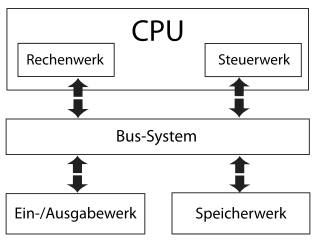
\includegraphics[width=4cm]{Von-Neumann_Architektur}
	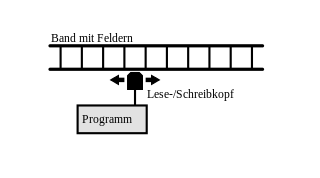
\includegraphics[width=6cm]{Turingmaschine}
	\caption{Von-Neumann, Turing-Maschine}
	\end{figure}
\end{card}

\begin{card}
	Im Zusammenhang mit dem Neumann-Rechnerkonzept ist die Rede vom von-Neumann-Flaschenhals, wenn Nachteile des Konzepts genannte werden.
	\begin{enumerate}[a)]
	\item Was ist darunter zu verstehen?
	\item Gibt es eine vergleichbare Problematik für die Turing-Maschine? 
	\end{enumerate}
	\hr
	\begin{enumerate}[a)]
	\item Alle Befehle / Daten müssen durch den Bus
	\item Schreib-/Lesekopf kann pro Zeiteinheit entweder schreiben oder lesen
	\end{enumerate} 
\end{card}

\begin{card}
	Nennen Sie wenigstens einen konzeptionellen Unterschied zwischen von-Neumann-Rechnerkonzept und Turing-Maschine.
	\hr
	Von TM ausgehend:
	
	\begin{itemize}
	\item Daten und Programme liegen \textbf{nicht} im selben Speicher
	\item keine Nummerierung/Adressierung eines Feldes auf dem Band
	\item keine Sprungadressen
	\item kann nur 1 Feld gehen pro Befehl
	\end{itemize}
\end{card}

\begin{card}
	Setzt die Turing-Maschine das von-Neumann-Rechnerkonzept um?
	\hr
	\textbf{Nein}, weil
	\begin{itemize}
	\item Bei TM: Daten $\neq$ Programme
	\item TM hat keine Sprungadresse
	\end{itemize}
	\vfill
	oder \textbf{Ja} mit Einschränkungen (vgl. Nein)
	\begin{itemize}
	\item Arbeiten befehlsorientiert
	\item Arbeiten deterministisch
	\end{itemize}
\end{card}

\begin{card}
	Wie könnte das Paradigma der strukturierten Programmierung in das von-Neumann-Rechnerkonzept integriert werden?
	\hr
	Überwachen bzw. Regeln der Sprunganweisungen.\\
	D.h. begrenzter Bereich (Scope) z.B. bei if-Anweisungen
\end{card}

\begin{card}
	Wieso verletzt das Konzept der lokalen static-Variablen in C das Paradigma der funktionalen
	Programmierung?
	\hr
	Funktionsausgabe nur abhängig von Eingabe. D.h. bei gleicher Eingabe gleiche Ausgabe (Idempotent, Deterministisch).
	\begin{lstlisting}[language=C]
	int f(int i) {
	  // Ausfuehrung bei Objekt-Init, 
	  // nicht bei Methodenaufruf
	  static int x = 0; 
	  x++;
	  return x+i;
	}
	\end{lstlisting}	
\end{card}

\begin{card}
	Wieso verletzen Pointer in C das Paradigma der funktionalen Programmierung?
	\hr
	Pardigma der f. Programmierung: Funktionsausgabe nur abhängig von Eingabe.  D.h. bei gleicher Eingabe gleiche Ausgabe.
	\begin{lstlisting}[language=C]
	int f(int *i) {
	  // Veraendern der Speicheradresse und 
	  //somit der Eingabe
	  *i = 1234;
	  ...
	}
	\end{lstlisting}	
\end{card}

\begin{card}
	In Java gibt es mit dem Collection-Framework eine Reihe von sogenannten Container-Klassen. Welches objektorientierte Programmierparadigma verletzen Objekte z.B. der Klassen	ArrayList oder Vector? 
	\hr
	Es werden Referenzen gespeichert. D.h. die Datenkapselung ist verletzt. Werte müssten unveränderlich (immutable) sein.
	\begin{lstlisting}[language=Java]
	class Dummy{int value;}
	...
	Dummy example = new Dummy()
	ArrayList<Dummy> list = new ArrayList<Dummy>()
	list.add(example);
	
	// Zugriff auf value ueber 2 Wege:
	example.value = 1;
	list.get(0).value = 2;
	\end{lstlisting}	
\end{card}

\begin{card}
	Wie müsste das Funktionskonzept in C beschränkt bzw. erweitert werden, damit es nicht zu Verletzungen des Paradigmas der funktionalen Programmierung kommen kann?
	\hr
	Zustandslosigkeit durch:
	\begin{itemize}
	\item kein static und Pointer 
	\item keine Systemaufrufe
	\end{itemize}
\end{card}

\begin{card}
	Das funktionale Programmierparadigma, das die referentielle Transparenz der Variablen fordert, wird in C durch die Zuweisung verletzt. 
	\begin{enumerate}[a)]
	\item Wie müssten die Regeln für die Verwendung der Zuweisung geändert werden, damit die	Zuweisung in das funktionale Konzept passt?
	\item Welcher Art von Anweisung entspräche die veränderte Zuweisung dann?
	\end{enumerate}
	\hr
	\begin{enumerate}[a)]
	\item Unveränderliche Variablen, Einmal-Zuweisung, bzw. nur Init.
	\item Konstanteninitialisierung
	\end{enumerate}
	
\end{card}

\begin{card}
	Die referentielle Transparenz sorgt dafür, dass Programme in rein funktionalen Sprachen	problemlos nebenläufig abgearbeitet werden können. 
	\begin{enumerate}[a)]
	\item Erklären Sie den Zusammenhang an einem Beispiel. 
	\item Erklären Sie an einem Beispiel den Zusammenhang fehlender referentieller Transparenz und Problemen bei nebenläufig ausgeführten Programmen. 
	\end{enumerate}
	\hr
	\begin{enumerate}[a)]
	\item Werte unveränderlich (immutable), d.h. kein Zustand und stark begrenzter Gültigkeitsbereich. Funktionen sind Thread-Safe, da Parameter nicht von außen geändert werden können.\\
	Beispiel: Immutable-Klassen sind automatisch thread-Safe, parallelisierbar und skalierbar. 
	\item Objekt-Parameter können während Thread-Unterbrechung über eine Referenz außerhalb der eigentlich Funktion verändert werden und haben somit einen anderen Zustand. Kein Determinismus, Race-Condition möglich.
	\end{enumerate}
\end{card}

\begin{card}
	Objektorientierte Sprachen kennen sogenannte inline-Funktionen.
	\begin{enumerate}[a)]
	\item Wieso sind inline-Funktionen in objektorientierten Programmiersprachen implementiert?
	\item Sind inline-Funktionen in rein funktionalen Programmiersprachen sinnvoll?
	\item Welches Problem ergibt sich aus inline-Funktionen im Rahmen einer rein funktionalen Sprache?
	\end{enumerate}
	\hr
	\begin{enumerate}[a)]
	\item Performancevorteile, da weniger Overhead ohne Heap / Stack.
	\item Ja, erhöhen Geschwindigkeit
	\item Rekursionen können nicht aufgelöst werden. Daher nur als Zusatz, nicht als Ersatz für normale Funktionen.
	\end{enumerate}
\end{card}

\begin{card}
	Angenommen in C würden innerhalb von parametrisierten Makros Zuweisungen nicht mehr	zugelassen sein.\\
	Inwiefern verletzen Makros dann trotzdem weiterhin Paradigmen der funktionalen Programmierung?
	\hr
	Variablen sind außerhalb vom Makro gültig, d.h vor oder nach dem Aufruf / Ersetzung.\\
	Durch die Textersetzung können Variablen(namen) genutzt werden, die erst im nachfolgenden Programm definiert werden. Dadurch ist Idempotenz / Determinismus verletzt.\\
	Beispiel:
	\begin{lstlisting}[language=C]
	#define printX print x
	int x = 100;
	printX(); // Ausgabe: 100
	\end{lstlisting}
\end{card}
\end{document}